\documentclass[12pt,a4paper]{article}

\usepackage[utf8]{inputenc}
\usepackage{graphicx}
\usepackage{pdfpages}
\usepackage{csquotes} % czech styled quotes 
\usepackage[czech]{babel} % czech babel 
\usepackage{mathtools} % math magic
\usepackage{amssymb} % some funky math symbols like \trinangleq
\usepackage[left=4cm,right=1.5cm,top=3cm,bottom=3cm]{geometry} % set smaller page borders 
\usepackage[indent=0pt]{parskip} % spaces between paragraphs, indents sets indent of the first line in paragraph
\usepackage{hyperref}
\usepackage{pdflscape}
\usepackage{enumitem}
\usepackage{caption}
\usepackage{subcaption}
\usepackage{fontspec}
\usepackage{unicode-math}
\usepackage{lmodern}
\usepackage{setspace}
\usepackage{titlesec}
\usepackage{float}

\usepackage{listings}
\usepackage{color}

\definecolor{dkgreen}{rgb}{0,0.6,0}
\definecolor{gray}{rgb}{0.5,0.5,0.5}
\definecolor{mauve}{rgb}{0.58,0,0.82}

\lstset{
	language=Python,
	showstringspaces=false,
	columns=flexible,
	basicstyle={\small\ttfamily},
	numbers=none,
	numberstyle=\tiny\color{gray},
	keywordstyle=\color{blue},
	commentstyle=\color{dkgreen},
	stringstyle=\color{mauve},
	breaklines=true,
	breakatwhitespace=true,
	tabsize=4
}

\setstretch{1.5}
\setmainfont[
	Extension=.otf,
	UprightFont={*-Regular},
	BoldFont={*-Bold},
	ItalicFont={*-Italic},
	BoldItalicFont={*-BoldItalic},
	% RawFeature={+zero}
]{LibertinusSerif}
\setmathfont{LibertinusMath-Regular.otf}

\graphicspath{{images/}}


\begin{document}

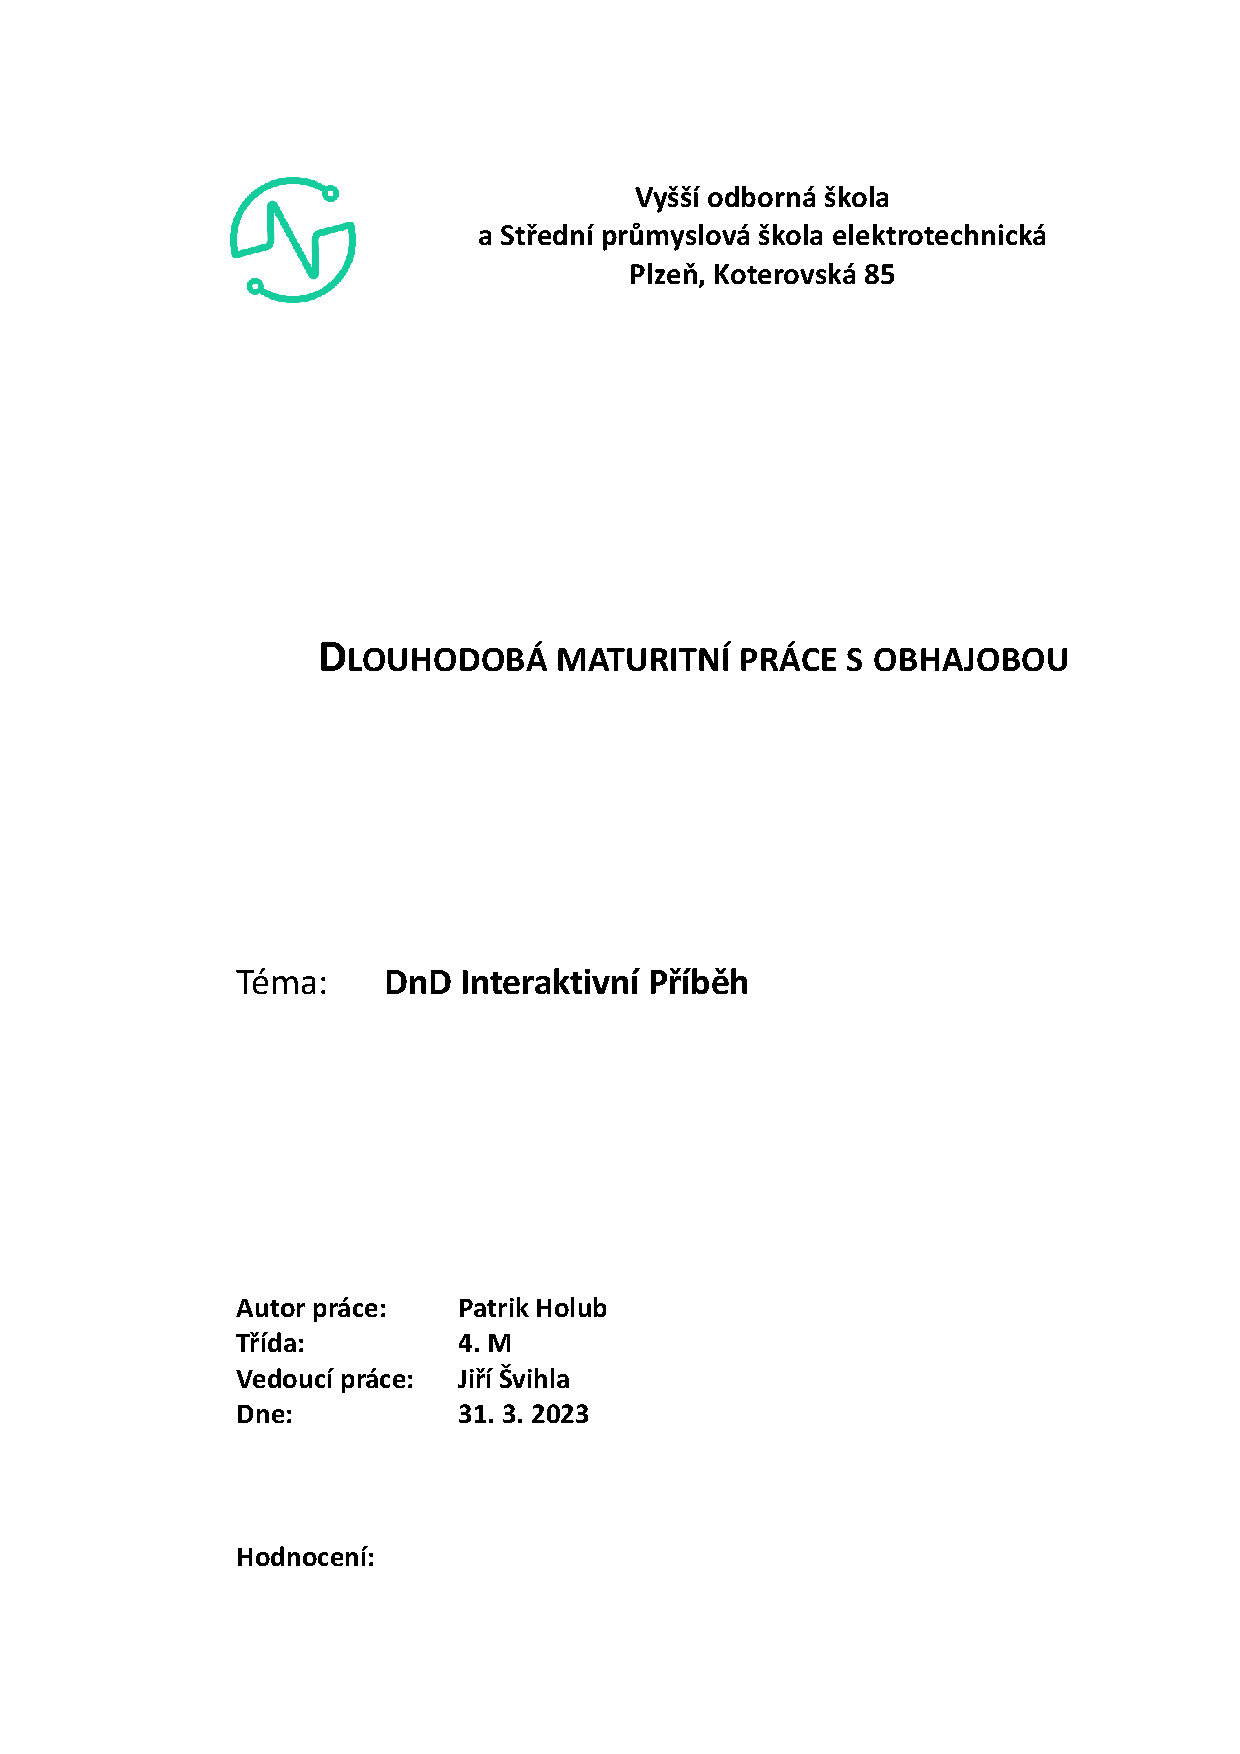
\includepdf[pages=-]{add_files/mp_titlelist}
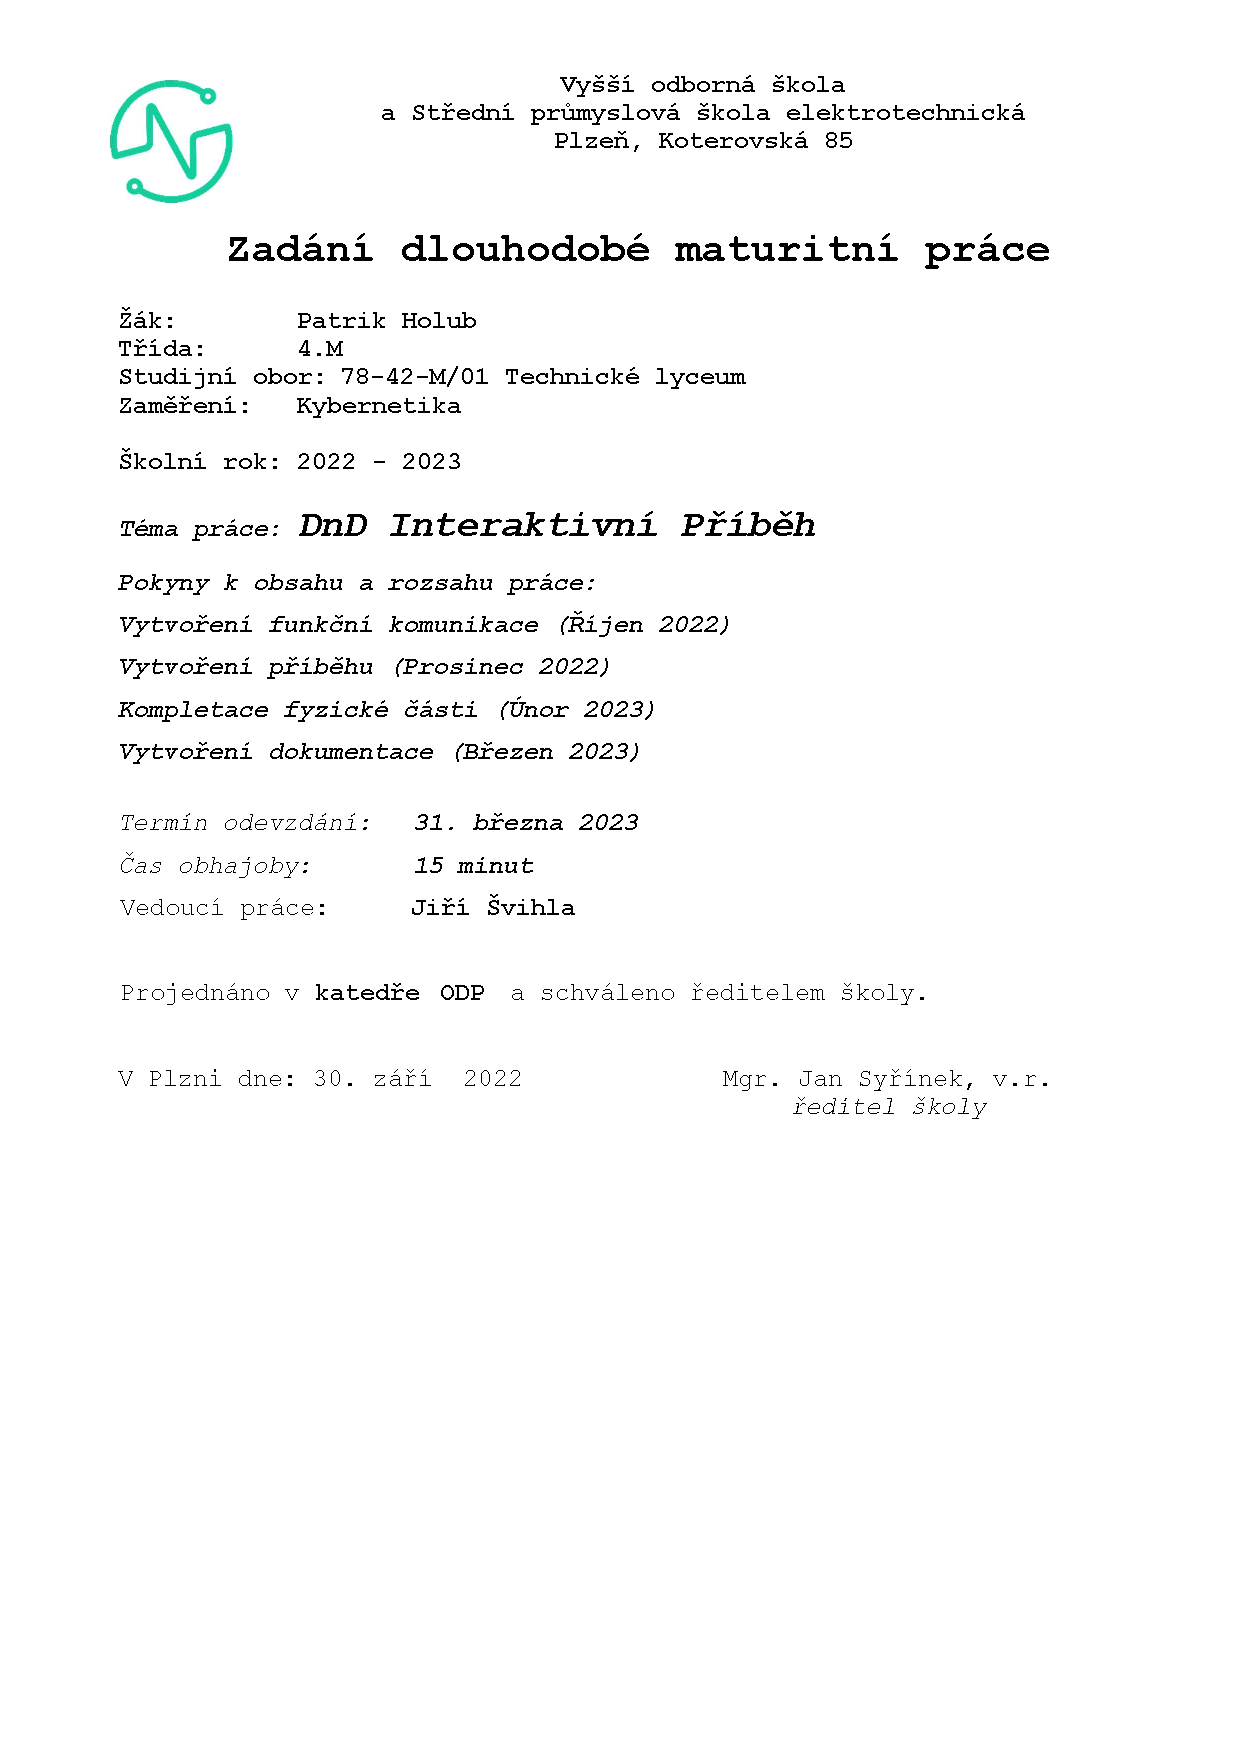
\includepdf[pages=-]{add_files/zadanibelike}

\newpage

\section*{Anotace}
V této maturitní práci se snažím o vytvoření programu který je schopný přednést příběh a předložit hráči možnosti na které příběh bude reagovat. Tímto se docílí interaktivita příběhu. Zároveň vše je děláno systémem skriptů, tudíž je možno hru, při dodržení pravidel pro psaní daných skriptů, měnit pomocí uživatelsky napsaných programů. Projekt také obsahuje metodu se kterou se dá zjednodušeně příběh napsat a použít jednotlivé skripty pro interaktivitu. Poslední část práce je uložení hráče a jeho odpovídajících skriptů na raspberry pi pico a čtení předem zmíněného obsahu ze zařízení. Celá práce je dělaná v programovacím jazyku Micropython.
%\addcontentsline{toc}{Anotace}{Anotace}


\vspace*{\fill}

„Prohlašuji, že jsem tuto práci vypracoval samostatně a použil(a) literárních pramenů a informací, které cituji a uvádím v seznamu použité literatury a zdrojů informací.“ 
„Souhlasím s využitím mé práce učiteli VOŠ a SPŠE Plzeň k výuce.“ 
\begin{flushright}
	V Plzni dne: …..................... Podpis: …..........................
\end{flushright} 

\newpage
\section{Fyzický klíč}
Pro komunikaci jsem vytvořil design vlastní desky, založené na čipu RP2040. Tato deska je schopná zobrazit informace ohledně hráče, pokud daná informace má min a max. 

Zobrazování je provedeno pomocí 8 LED na každé straně, které jsou ovládaný přes 8 bitový posuvný registr v časovém multiplexu pro ovládání dvou stran zároveň. Tento časový multiplex běží rychlostí 2kHz aby každá strana běžela na rychlosti 1kHz. Zvolená rychlost byla ze dvou důvodů. První byl, že při takové rychlosti by oko nemělo být schopné zaznamenat jak strany blikají. Druhý důvod souvisí s frekvencí na které často běží PWM. Díky těmto vlastnostem jsem schopný ovládat LED buď aby jenom blikali, nebo abych ovládal jejich jas pomocí simulovaného PWM.  
\subsection{Komunikace}
Máme dvě komunikační zařízení a potřebujeme vytvořit komunikaci mezi nimi. Komunikace je řešena přes comporty. Hostitel, v tomto případě počítač, na kterém běží hlavní program, si nechá pomocí nástrojů knihovny serial vypsat všechny rozpoznané comporty. Následně se pokusí otevřít comport a poslat mu příkaz. Pokud se mu nepovede otevřít comport, víme že je to nechtěné zařízení. Když se otevření povede, pošle mu příkaz "type". Pokud je na druhé straně správné zařízení neboli pico se správným nahraným programem, tak zpátky odešle zprávu "player". Jenom tehdy je zařízení dáno do listů zařízení, se kterým potom program pracuje dál.

Hostitelský program je o dost složitější než ten na picu. Hostitel musí zprávu nejdřív převést do kódování utf-8 neboli bytes. To je posláno na sériovou linku comportu, který je zrovna otevřený. Pico má práci velmi jednoduší, neboť micropython je schopný číst sériovou linku pomocí příkazu input(). Následně pico kontroluje jakou zprávu dostal vůči svému slovníku. Pokud zpráva odpovídá nějakému příkazu, tak pico navrátí odpovídající hodnoty, jinak jenom pošle zpět že zprávu zaregistroval. Hostitel nyní musí projít zpětným procesem převádění zpět z bytes na string. Pokud pico pošle víceřádkovou správu, tak samozřejmě musí komunikační program převést celé pole, které přečte z comportu. 

\subsection{Datová struktura}
Díky způsobu práce s daty na klíči (nepracuje s nimi přímo uživatel, vše je ovládáno pomocí programu) tak zde může existovat velmi neflexibilní struktura souborů. V rootu musí existovat main.py, který se sám spustí, když se pico zapojí. Zároveň musí být v rootu samotný soubor hráče a jakékoli knihovny, které main.py potřebuje. Následně všechny skripty, které jsou specifické vůči hráči, musí být v adresáři player\_scripts.

\newpage
\section{Struktura adresářů a souborů}
Během tvorby programu byl kladen důraz na co nejméně vynucené struktury ze strany uživatele. Hodně problémů jsem tudíž vyřešil pomocí tvorby souborů se specifickými názvy, pro které se program dívá a vytvoří si strukturu cest, se kterou pracuje a podává do dalších funkcí. Je zde ale určitá kultura, kterou bych doporučil při tvoření souborů.

Hlavní adresář příběhu
\begin{itemize}
	\item Soubor s názvem "\_story.txt"
	\item Adresář s inicializačními skripty
	\item Adresář se skripty eventů
	\item Adresář s hráči (může být prázdný, pokud je použit klíč)
	\item Adresář se skripty hráčů 
	\item player\_scripts
	\item další adresáře, které už tvoří vlastní strukturu příběhu
\end{itemize}

Všechny adresáře, které obsahují skripty, musí obsahovat soubor "\_scripts.txt" a "info.json". První soubor je hledán aby program věděl kde má skripty uložené a druhý soubor obsahuje informace pro program jak se jednotlivé skripty chovají.

Jednotlivé části příběhu, se kterými chceme aby program pracoval, jsou určeny soubory "storypart.json". Tento soubor obsahuje jednu informaci pro program, "include" určující obsáhnutí při prvotním načtení, a dále jakékoli další informace, se kterými chce následně uživatel pracovat ve svých skriptech.

Jedno místo kde program nehledá pro "storypart.json" jsou soubory, které začínají tečkou. Doporučuji u každého "storypart.json" vytvořit adresář .orig, který obsahuje původní stav celého adresáře. Logické skripty, které vysvětlím později, mají schopnost měnit soubory přímo a nelze je vrátit na původní stav, pokud uživatel nezná původní stav.


\section{Hlavní program}
Vše je psáno pomocí programovacího jazyka Python, přičemž velmi využívám datového souboru typu json pro ukládání rozmanitých dat.

Hlavní program nastaví všechny iniciální hodnoty, provede inicializační sekvenci, najde místo příběhu a najde všechny eventy, které se budou muset stát. Všechny eventy mají své odpovídající skripty a hlavní program samozřejmě provede jejich import. Zároveň vytvoří list importovaných funkcí aby s nimi metody a funkce mohli pracovat.

Jako poslední, hlavní program samozřejmě obsahuje smyčky pro průběh programu.

\subsection{Handler}
Nejdůležitější součást programu je handler. Tato funkce je schopná vzít script a odpovídající parametry, dosadit hodnoty z paměti, funkci zavolat a uložit její návratovou hodnotu. 

Handler jako funkce má dva svoje parametry. První parametr musí být název skriptu bez koncovky .py (takto jsou uloženy v naimportovaných skriptech). Druhý parametr je pole argumentů, které chceme do funkce poslat. Handler používá vybalovací znaménko * aby první dimenze pole byla předána funkci jako jednotlivé parametry. Zároveň se v této první dimenzi hledá \& znak, který jsem zvolil jako identifikátor že je třeba vzít hodnoty z paměti. Pokud nějakou najde hodnotu v paměti, nahradí \& znak odpovídající hodnotou.

Dalším krokem je zavoláním funkce. Hlavní program obsahuje list importovaných funkcí, a protože Handler žije uvnitř hlavního programu, tak může sáhnout do tohoto listu a funkci zavolat. Volání funkce je provedeno přes funkci getattr().

Zpracování návratových hodnot vyžaduje správné zapsaní informací v "info.json" souborech, které si program načte do paměti. Tyto soubory mají strukturu slovníku a obsahují dvě sekce. První sekcí, jménem id, je soupis názvů skriptů a jejich id. Druhá sekce, jménem info, je určená jak pro důležité programové informace tak pro uživatelské. Dva programové listy které se zde nacházejí jsou pod klíči "func" a "obj". Každá funkce se musí nacházet v jedné z nich a ne v obou zároveň. Handler zjišťuje jestli funkce vrátila hodnotu, pokud ano tak ji ukládá do paměti. Pokud ale skript neobsahuje funkci, obsahuje objekt, tak handler zavolal konstruktor a musí se tudíž celý objekt uložit do paměti.

Mezi další, již nepovinné, informace patří například listy pod klíči "lock" a "logic". První pole říká handlerovi aby hodnotu, kterou načetl z paměti nezahazoval a ponechal ji v paměti. Jsou to tudíž "zamčené" hodnoty. Tato možnost by měla být použita pouze pro skripty u kterých víme že nebudou volány více než jednou. Nebo pokud víme že následně v eventech budou hodnoty násilně požrány. 

Druhý list určuje takzvané logické skripty. Pokud je jejich návratová hodnota typu slovník, mají schopnost přidávat eventy a tudíž jsou logické skripty schopné vytvářet smyčky. Kromě návratových hodnot typu slovník handler také u rozpoznává stringy s koncovkou .json. Pokud je takový string nalezen, tak Handler z odpovídajícího souboru vezme eventy a přidá je. Handler je ještě schopný nalézt jeden identifikátor, "self". Pokud je "self" nalezen a jeho hodnota je true, tak handler přidá, celý původní script, který byl volán. Toto umožňuje snadno vytvořit nekonečnou smyčku.
\subsubsection{Paměť programu}
Struktura paměti je takzvaný stack. Pro tento účel jsem vytvořil třídu, abych si mohl dodat manipulační metody, které bych mohl potřebovat. Samotný stack má strukturu listu (toto jsem zvolil abych mohl použít indexované hledání, mazání, či přidávání hodnot), kdy hodnotou listu je vždy list o dvou hodnotách. Na první pozici stojí vlastní hodnota a na druhé stojí id, neboli adresa, funkce či objektu, co tuhle hodnotu vytvořila. Pokud funkce chce pracovat s hodnotami jiných funkcí, tak je použita první nalezená hodnota "shora" (Pokud bychom se dívali na hodnoty od indexu 0 až do X, tak by to byla první hodnota nalezená od nuly).

Pro manipulaci hodnot jsem vytvořil také dva skripty, které může uživatel používat a to je putVal, pushVal a eatVal. PutVal jednoduše přidá hodnotu do stacku pod svojí vlastní ID. PushVal je schopný posunout hodnotu na na další místo ve stacku za nejbližší hodnotu se stejnou adresou. EatVal požere hodnotu ze stacku i za možnosti že je to "uzamčená" hodnota.

Jak jsem již zmiňoval v sekci Handler, pro čtená z paměti jsem vybral znak \&. Inspiroval jsem se z programovacího jazyka C kde \& operátor vrací adresu proměnné. V mém případě je za znakem \& adresa kde se hodnota má nacházet v paměti.
\subsubsection{Struktura Scriptu}
Kvůli použití funkce getattr() ve funkci Handler, a zjednodušení programu, má script jedno nutné
pravidlo, které se musí dodržovat. Script vždy musí obsahovat stejnojmennou funkci jako soubor, ve kterém je obsáhlá. Na první pohled se toto zdá jako divné pravidlo a vytvoří to velmi elegantní zápis: 
\begin{lstlisting}[language=Python] 
volana_funkce = getattr(importy[funkce],  funkce) 
\end{lstlisting}
\subsection{Okno Hry}
\subsubsection{Formátování}
\subsubsection{Vytváření a práce s oknem}
\subsection{Tělo Hry}
Tělem hry je zde míněno celková struktura, která tvoří herní zážitek.
\subsection{Struktura příběhu}
\subsection{Eventy}
\subsubsection{Zápis eventů}
\subsubsection{Popisové informace}




\end{document}